\documentclass[10pt,conference]{IEEEtran}
%\documentclass[conference]{ieeetran}
\IEEEoverridecommandlockouts
% The preceding line is only needed to identify funding in the first footnote. If that is unneeded, please comment it out.
%\usepackage{
\usepackage{verbatim}
\usepackage{amsmath,amssymb,amsfonts}
\usepackage{algorithmic}
\usepackage{textcomp}
\usepackage{floatrow}
\usepackage{xcolor}
\def\BibTeX{{\rm B\kern-.05em{\sc i\kern-.025em b}\kern-.08em
    T\kern-.1667em\lower.7ex\hbox{E}\kern-.125emX}}

\usepackage{caption}
\captionsetup[table]{skip=0pt,singlelinecheck=off}

\usepackage{graphicx}
\graphicspath{ {./res/} }

\usepackage{hyperref}
\usepackage{float}
\usepackage{minted}
%\usepackage{flushend}

\newcommand{\norm}[1]{\left\lVert#1\right\rVert}

\begin{document}

\title{Semantic-based Anomaly Index for \\ Source Code}

\author{\IEEEauthorblockN{
%Akimova E.N.\IEEEauthorrefmark{1}\IEEEauthorrefmark{2},
%Bersenev A.Yu.\IEEEauthorrefmark{1}\IEEEauthorrefmark{2},
%Cheshkov A.S.,
%Deikov A.A.\IEEEauthorrefmark{1}\IEEEauthorrefmark{2},
%Kobylkin K.S.\IEEEauthorrefmark{1}\IEEEauthorrefmark{2},\\
%Konygin A.V.\IEEEauthorrefmark{1},
%Mezentsev I.P. \IEEEauthorrefmark{1}\IEEEauthorrefmark{2}, and
%Misilov V.E.\IEEEauthorrefmark{1}\IEEEauthorrefmark{2}}
% \IEEEauthorblockA{
%\IEEEauthorrefmark{1}N.N. Krasovskii Institute of Mathematics and Mechanics\\
%\IEEEauthorrefmark{2}Ural Federal University\\
%Ekaterinburg, Russia \\
%Email:
%aen@imm.uran.ru,
%alexander.bersenev@urfu.ru,
%acheshkov@gmail.com,
%deykov.artem@urfu.ru,\\
%kobylkin@imm.uran.ru,
%konygin@imm.uran.ru,
%ilya.mezentsev@urfu.ru,
%v.e.misilov@urfu.ru
}}
\maketitle

\begin{abstract}
The software development community has been using handcrafted code quality metrics for a long time.
Despite their widespread use, these metrics have a number of known shortcomings.
The metrics do not take into account project-specific coding conventions, the wisdom of the crowd, etc.
To address these issues, we propose a novel semantic-based approach to calculating an anomaly index for the source code.
This index called {\sc A-Index} is the output of a model trained in unsupervised mode on a source code corpus.
%The model is based on Transformer and variational autoencoder.
The larger the index value, the more atypical the code fragment is.

To test {\sc A-Index} we use it to find anomalous code fragments in Python repositories.
Also, we apply the index for a variant of the source code defect prediction problem.
Using BugsInPy and PyTraceBugs datasets,
we investigate how {\sc A-Index} changes when bug code is fixed.
The experiments show that in 63\% of cases, the index decreases when the bug is fixed.
If one keeps only those code fragments for which the index changes significantly,
 then in 71\% of cases the index decreases when the bug is fixed.
%The experimental results demonstrate the usefulness of the proposed approach in the task of defect prediction.
\end{abstract}


\begin{IEEEkeywords}
anomaly detection, code quality, defect prediction
\end{IEEEkeywords}


\section{Introduction}\label{intro}

Source code metrics are an important part of the software measurement process.
As a rule, they are calculated from the source code and allow one to characterize it.
Despite their widespread usage, work is still ongoing to develop new metrics \cite{SharmaSpinellis2020}.

Metrics can be used as indicators or as features for code representation (embeddings).
In addition, metrics can be {\it explicit} ({\it traditional} or {\it handcrafted}) or {\it implicit} \cite{NunezVarelaEtAl2017}, \cite[Appendix]{AfricEtAl2020}.
Explicit metrics can be interpreted, but at the same time have known drawbacks,
 since they are invented by a human and implemented as an algorithm.
Implicit metrics are usually poorly interpreted, but capable of capturing complex non-obvious patterns.
In addition, implicit metrics are able to adapt to the data on which they were trained.
One of such problems where implicit metrics can be more efficient than handcrafted is the problem of defect prediction \cite{AkimovaEtAl2021}.
Defect prediction is one of the key challenges in software development.
Any new advances in the problem are welcome as they can lead to better code quality and software reliability.
Usually, defect prediction problem is posed as a classification problem with two classes:
 code with defects and code without defects \cite{AllamanisEtAl2018}.
Since the class with defective code is small, there is a class imbalance problem \cite{AlsawalqahEtAl2017}.
One way to tackle the issue is to consider a defective code as a kind of anomalous one.
The work \cite{RayEtAl2016} demonstrates that it is not only convenient, but also quite natural to consider a defective code anomalous.
The authors find that code with bugs tends to be more entropic (i.e. unnatural), becoming less so as bugs are fixed.

In this work, we propose a unsupervised semantic-based approach to calculating anomaly index for source code.
The higher the index is, the more likely a code is atypical.
We use the resulting anomaly index to find anomalous Python code and present some found code fragments.
In addition, we use this index for one of the variants of the source code defect prediction problem.
We show on bug-fix datasets BugsInPy, PyTraceBugs, that the anomaly index of the fragment decreases when the bug is fixed.

Contribution:
\begin{itemize}
\item  we present an unsupervised semantic-based approach to calculating the implicit anomaly index for the source code;
\item  we detect atypical code in Python code;
\item  we evaluate this index on the bug-fix datasets.
\end{itemize}


\section{Related work}\label{related}

{\it Anomaly detection} is the identification of data that is significantly different from most other data.
Typically, abnormal data indicates a specific type of problem, such as banking fraud, structural defect, health problems.

With regard to software development, anomaly detection is used, for example, to detect vulnerabilities in programs \cite{FengEtAl2003, GonzalezEtAl2021}.
Anomaly detection for logs is used to diagnose deviations in the programs \cite{HashemiMantyla2021a, HashemiMantyla2021b}.
The architecture impact of a wide range of code-anomaly agglomerations is studied in \cite{OizumiEtAl2015}.
One of the popular applications of the anomaly detection problem is defect prediction.
Due to the imbalance of the classes, such an application seems natural.

The closest to our work is \cite{RayEtAl2016}, where the authors investigate the hypothesis that unnatural in some sense code is suspicious.
For this, a modified $n$-gram language model is constructed, which estimates the conditional probability of the next token appearance.
Thus, the approach allows you to find code that is unnatural (has a low probability) from the point of view of the language model.
Since the language model deals with syntax, code containing syntactic anomalies would be unnatural.
In our approach, anomaly is estimated in the semantic contextual multilingual representation space.
Instead of taking syntactic-level structure of code, the representation uses data flow in the pre-training stage,
 which is a semantic-level structure of code \cite{GuoEtAl2021}.

In \cite{NeelaEtAl2017}, the authors use explicit features and the Gaussian distribution to model nondefective code,
 and defective code is then predicted using the deviation from the model estimation.
The possibility of using explicit features and the $k$-nearest neighbors algorithm
  for the anomaly detection in the source code is demonstrated in \cite{MoshtariEtAl2020}.
In \cite{TongEtAl2018}, the stacked denoising autoencoders \cite{VincentEtAl2010}
 are used to extract deep representations from the traditional software metrics.
A similar idea is implemented in \cite{SakuradaYairi2014} and  \cite{AfricEtAl2020}
 where the autoencoder on the explicit features is used for within-project source code anomaly detection.
In \cite{BryksinEtAl2020}, two approaches to code vector representation are implemented:
 a feature vector consisting of $51$ explicit code metrics and an implicit $n$-gram approach.
Additionally, several anomaly detection techniques are tested:
 local outlier factor, isolation forest, and autoencoder neural network.
The authors focus on two types of anomalies: syntax tree anomalies and compiler-induced anomalies in the Kotlin code.
The found fragments of anomalous code are used by the developers of the Kotlin compiler for more efficient testing \cite{BryksinEtAl2020}.

One more reason for using anomaly detection for defect prediction is the possibility of using unsupervised learning \cite{AllamanisEtAl2021}.
It is both time-consuming and labor-intensive to create a big labeled dataset,
while modern machine learning approaches require a lot of data.
And in many settings labeled data is much harder to come by than unlabeled data.

Before moving on to the description of our approach, it is necessary to say a few words about the representation of the code.
A code representation is a mapping of a code fragment into a feature vector.
At the moment, there are various ways to implicitly represent the code.
These representations differ in the underlying architecture and the types of tasks on which the training took place:
 e.g. code2vec \cite{AlonEtAl2019vec}, code2seq \cite{AlonEtAl2019seq}, PathPair2Vec \cite{ShiEtAl2020}, CuBERT \cite{KanadeEtAl2020}, CodeBERT \cite{FengEtAl2020},
 and GraphCodeBERT \cite{GuoEtAl2021}.
In the current work, we use GraphCodeBERT, because in addition to using the task of masked language modeling,
 it uses two structure-aware pre-training tasks.
One is to predict code structure edges, and the other is to align representations between source code and code structure. 


\section{Proposed approach}\label{approach}

The concept of anomaly depends decisively on the probabilistic space under consideration and on the source code corpus used.
The choice of the corpus is determined by the problem to be solved.
In this work, we use a set of different repositories as a corpus (see below for details).
The general scheme of the approach is shown in Fig. \ref{approach}. All steps are described in more detail below.

\begin{figure}[htbp]
\caption{{\sc A-Index} overview:
The source code of the programs is split into fragments.
Each of the fragments is converted to a fixed-dimensional vector using a Transformer-based model.
These vectors are the input to the variational autoencoder.
The reconstruction error is the resulting value of the anomaly index.}
\centering
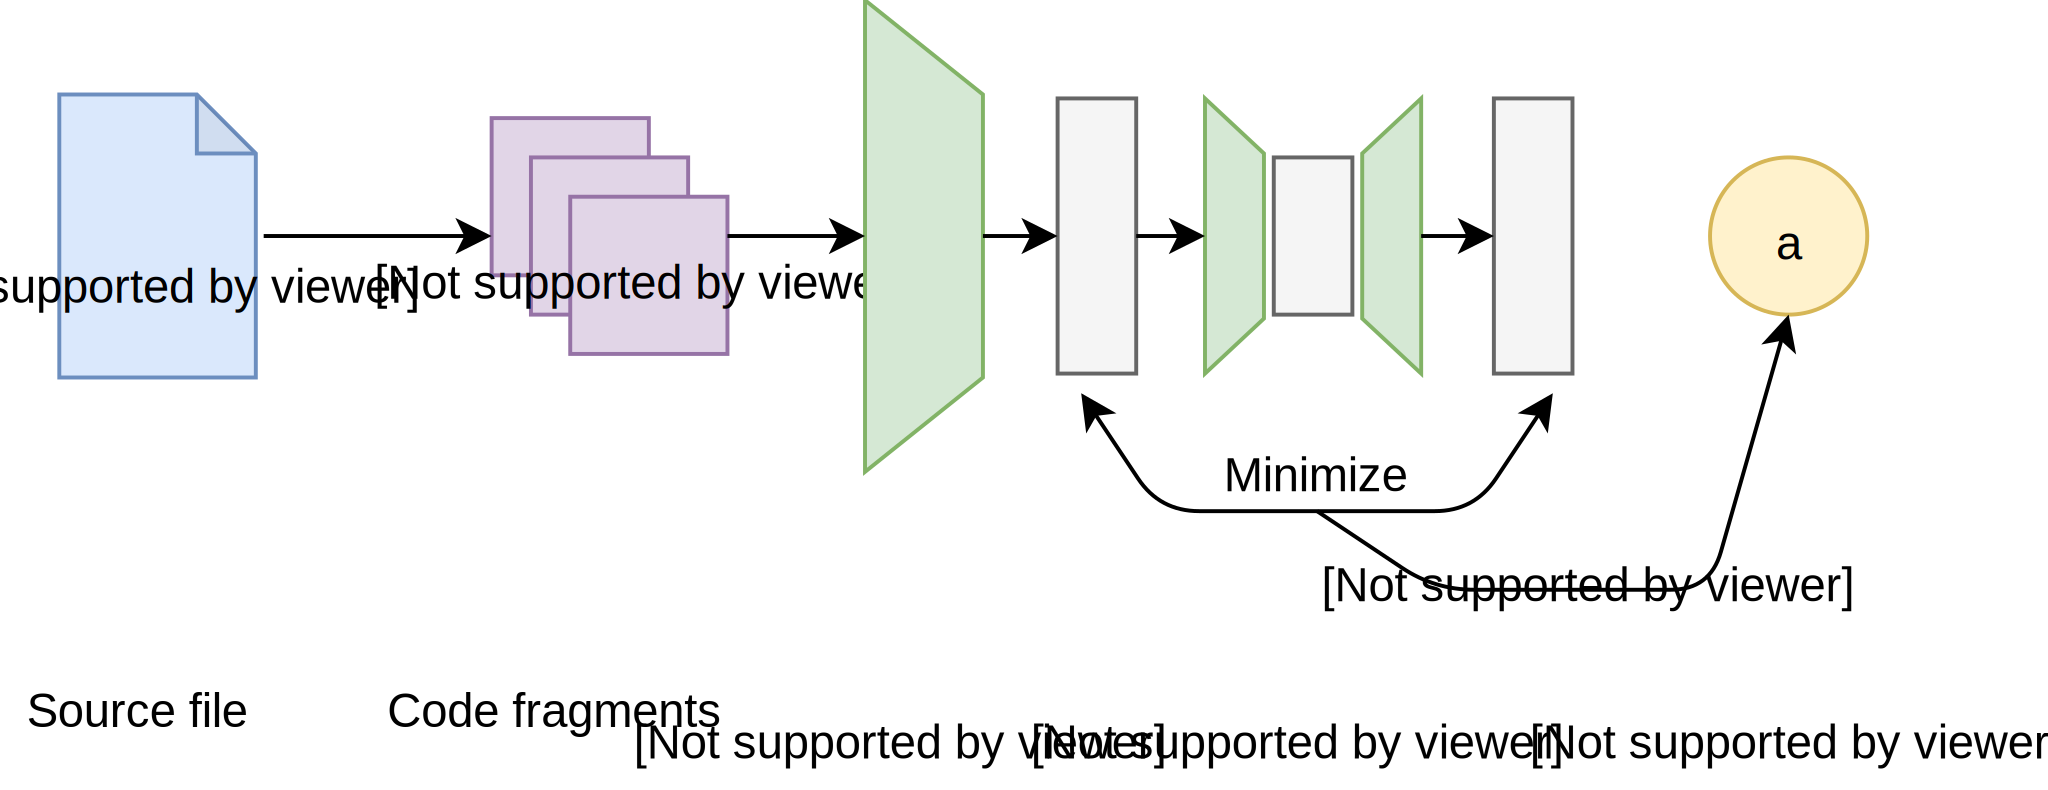
\includegraphics[width=1.0\textwidth]{approach}
\label{approach}
\end{figure}

Before moving on to the details of our implementation, let's list the main steps we need to take:
\begin{enumerate}
\item Choose code corpus and level of granularity.
\item Transform code fragments into vectors from $R^n$, where $n$ is the fixed dimension of the representation space.
\item Train an anomaly model.
\end{enumerate}


{\bf Code corpus.}
We use an unlabeled source code corpus, which leads us to unsupervised methods.
Our current work uses the Py150 corpus \cite{RaychevEtAl2016},
 which consists of the Python programs, collected from the GitHub\footnote{https://github.com/} repositories
 by removing duplicate files, removing project forks (copy of another existing repository),
 and keeping only programs that have no more than 30,000 nodes in the abstract syntax tree.
Furthermore, only repositories with the permissive and non-viral licenses such as MIT, BSD, and Apache are used.
The dataset is split into two parts 100,000 files used for training and 50,000 files used for evaluation. 
Also we use the Django repository\footnote{https://github.com/django/django} for within-project anomaly detection.
  
The anomaly index is calculated for a fragment of the source code.
Therefore, each corpus file needs to be converted into a set of fragments.
In this work, individual functions act as code fragments.

Before proceeding with the description of the code representation,
 it is necessary to make a note about the choice of the corpus.
If the index is supposed to be used within the framework of one project, then this project or a part of it should be such a corpus.
The main requirement for the choice of the corpus is its representativeness.
The corpus should be large enough to accommodate various coding conventions, the wisdom of the crowd, etc.


{\bf Code representation.}
The proposed approach uses GraphCodeBERT \cite{GuoEtAl2021} representation for code fragments.
It is a pre-trained model for a programming language that considers the inherent structure of code.
GraphCodeBERT is semantic contextual multilingual representation based on the multi-layer bidirectional Transformer \cite{VaswaniEtAl2017}.
The model follows BERT \cite{DevlinEtAl2019} and RoBERTa \cite{LiuEtAl2019}.
The resulting $768$-dimensional vector represents code fragment.


{\bf Anomaly model.}
For anomaly detection the model uses variational autoenconder (VAE, for details, see \cite{KingmaWelling2014, RezendeEtAl2014}).
In the variational autoencoder, the loss function is composed of two parts:
 the $L_2$-loss (reconstruction loss) and Kullback --- Leibler divergence (latent loss, \cite[Appendix B]{KingmaWelling2014}):
$$\norm{X - f(z)} + D_{\mathrm{KL}}\big(\mathcal{N}(\mu(X), \Sigma(X) ) ~||~ \mathcal{N}(0, I)\big).$$
In this formula, we use the standard notation from \cite{KingmaWelling2014}.
The first part tends to make the encoding-decoding scheme as precise as possible.
The second part tends to regularize the organization of the latent space by making the distributions
 returned by the encoder close to a standard normal distribution.
Unlike other autoencoders that represent each value of the encoding with a single value,
 the variational autoencoder learns to represent it as latent distributions
 and can approximate by virtue of the Bayesian inference.
This means that a variational autoencoder is more appropriate than a simple autoencoder for the extrapolation tasks.
The parameters of our variational autoencoder were learned with respect to the Gaussian distribution.
The hidden size of the autoencoder is a hyperparameter whose values belong to the set
 $\{4, 8, 16, 32, 64, 128\}$.

To calculate {\sc A-Index}, we use the reconstruction error term.
The larger this error, the worse the code fragment matches the probabilistic model of the variational autoencoder.
{\sc A-Index} can be viewed as some kind of code quality metric.
Unlike the standard metrics, the index is implicit and depends significantly on the corpus by which the underlying model is trained.
The ability of the index to adapt to a specific repository expands the possibilities of its usage.


\section{Results}\label{results}

We carried out some experiments to study the properties of the index.
Each experiment corresponds to a research question (hereinafter RQ).

\bigskip

%{\bf Cross-project anomalous code detection.}
%The first experiment is to detect atypical fragments in the source code corpus.

\begin{quote}\emph{RQ1: Can A-Index be used to detect suspicious code?}\end{quote}

We train {\sc A-Index} using Py150.
The Py150 train/test split provides approximately $641,000$ code fragments in training and approximately $314,000$ code fragments in testing.
Every fragment is represented by a $768$-dimensional vector (embedding).
The training was not required to obtain such a representation, since we were already using a model with pre-trained weights. 
However, the proposed approach leaves room to fine-tune the code representation model for downstream tasks.
The training of VAE takes over $200$ epochs using Adam \cite{KingmaBa2015} with a learning rate of $0.001$ 
 and batch size of $128$ as an optimization algorithm.

To answer RQ1, we apply the index to detect anomalous (atypical) code fragments in the test part of the Py150 corpus.
Recall that the larger the reconstruction error, the more likely the code fragment is atypical.
Thus, the analysis of code fragments with a high index value gives an answer to the question
 whether it is possible to find suspicious code using the proposed approach or not.
With thin analysis we found, that among the fragments that got a large {\sc A-Index} value, there are many one-line functions that do not implement any logic,
 use bitwise operations, string variables, and non-standard constructs.

Due to the natural limitations on the size and number of fragments,
 we present here only a few examples of compact functions that have received a large index value.
One-line examples are shown in Fig. \ref{oneline},
 and some examples of compact functions among the most anomalous are shown in Fig. \ref{compact}.

\begin{figure}[H]
\caption{Samples of one-line functions among the most anomalous in the Py150 corpus}
\label{oneline}
\begin{minted}[fontsize=\footnotesize, %frame=lines,
               mathescape,
               framesep=5mm]{python}
def Pop(): pass

def __UINT64_C(c): return c ## UL

def supportedExtensions():
    return ['.bmp', '.jpg', '.jpeg', '.png']

def GetRValue(rgb): return rgb & 0xff

def setPlayerInvItemNum(index, invSlot, itemNum):
    Player[index].char[TempPlayer[index].charNum].\
    inv[invSlot].num = itemNum

def tzname(self, dt):                                                                                                                                     
    return self._name
\end{minted}
\end{figure}

\begin{figure}%[H]
\caption{Samples of compact functions among the most anomalous in the Py150 corpus}
\label{compact}
\begin{minted}[fontsize=\footnotesize, %frame=lines,
               mathescape,
               framesep=5mm]{python}

def setExposure(value):
    global exposure
    exposure = value

def isValid( self ) :
    try :
        self.__dictEntry()
        return True
    except :
        return False

def __init__(self,X,K):
    self.X=np.array(X)
    self.K=K
    self.labels=[]
    self.centroids=[]
    pass
\end{minted}
\end{figure}

Despite the fact that among the found functions there are quite normal ones,
 many functions with a large value of the anomaly index are not ideally implemented.
The $\mathrm{Pop()}$ function does not implement the expected logic,
the $\mathrm{setExposure()}$ function modifies the global variable $\mathrm{exposure}$
 and requires careful handling.

Thus, using the index allows you to detect (perhaps not all) code fragments that, in our opinion, are suspicious.
Timely detection of such code fragments (for example, during the review stage),
 can improve the quality of the code and the reliability of the program.

\bigskip

%{\bf Within-project anomalous code detection.}

\begin{quote}\emph{RQ2: Can A-Index be useful within one separate repository?}\end{quote}

In the previous experiment the model is trained and applied to several repositories at once.
To answer RQ2, we train the model on the Python files of the Django project repository.
The trained model is applied to the test part of the same repository.

Since the listings of functions take up a lot of space,
 in this case we will only limit ourselves to the five functions (see Fig. \ref{five}) that have received the highest value of the anomaly index.

\begin{figure}%[H]
\caption{The functions than have received the highest score among the test part of the Django repository}
\label{five}
\begin{minted}[fontsize=\footnotesize, %frame=lines,
               mathescape,
               framesep=5mm]{python}

def duration_microseconds(delta):
    return (24 * 60 * 60 * delta.days +\
        delta.seconds) * 1000000 +\
        delta.microseconds

def etag(etag_func):
    return condition(etag_func=etag_func)

def b64_encode(s):
    return base64.urlsafe_b64encode(s).strip(b'=')

def last_modified(last_modified_func):
    return condition(last_modified_func=\
        last_modified_func)

def phone2numeric(phone):
    """Convert a phone number with letters into its\
    numeric equivalent."""
    char2number = {
        'a': '2', 'b': '2', 'c': '2', 'd': '3',
        'e': '3', 'f': '3', 'g': '4', 'h': '4',
        'i': '4', 'j': '5', 'k': '5', 'l': '5',
        'm': '6', 'n': '6', 'o': '6', 'p': '7',
        'q': '7', 'r': '7', 's': '7', 't': '8',
        'u': '8', 'v': '8', 'w': '9', 'x': '9',
        'y': '9', 'z': '9',
    }
    return ''.join(char2number.get(c, c)\
        for c in phone.lower())
\end{minted}
\end{figure}

While these functions appear to be correct, some of them nevertheless require special attention.
Thus, we conclude that the model can help find such code, and, therefore, can be useful for application within a separate repository.

\bigskip

We saw above that the model helps to find suspicious code,
 but is there a connection between the value of the anomaly index and the presence of a bug in the code?
In \cite{RayEtAl2016}, it was shown that from the point of view of the syntactic language model,
 the defective code is less natural than the bug-free code.
Below we will raise this question again, but for our model, which works in the space of semantic code representation.

\begin{quote}\emph{RQ3: Is there a connection between the value of the A-Index
 and the presence of a bug in the code?}\end{quote}

%The second experiment is an application of the index for differentiating bugs and fixes in bug-fix pairs.
To answer RQ3, we study how {\sc A-Index} is related to the presence of bugs or defects in code.
To do this, we use two available Python datasets.
Each of the datasets contains bug-fix pairs: a code fragment with a bug and its fixed version.
Our aim is to check how {\sc A-Index} changes when the bug is fixed.

The first dataset BugsInPy \cite{WidyasariEtAl2020} contains 493 real-life bugs.
Since our implementation of the index works at the function level,
 we dropped the pairs, that have several functions changed.
The second dataset PyTraceBugs (in the process of being published) is much larger.
It contains about 24 thousand bug-fix pairs, automatically collected from the GitHub platform.

The evaluation occurs as follows.
We learn 6 anomaly detection models with different sizes of the hidden layer: $4$, $8$, $16$, $32$, $64$, and $128$.
Each such model $M$ gives its own version of the index $a_M$.

For given model $M$ and dataset $D$,
 we take bug-fix pair $(c_{\mathrm{bug}}, c_{\mathrm{fix}})$ and calculate the anomaly index values: $a_M(c_{\mathrm{bug}})$ and $a_M(c_{\mathrm{fix}})$.
Next, we set a certain threshold $t$.

Let $$P := \{(c_{\mathrm{bug}}, c_{\mathrm{fix}}) ~\big|~ a_M(c_{\mathrm{bug}}) - a_M(c_{\mathrm{fix}}) \geq t\},$$
    $$U := \{(c_{\mathrm{bug}}, c_{\mathrm{fix}}) ~\big|~ |a_M(c_{\mathrm{bug}}) - a_M(c_{\mathrm{fix}})| < t\},$$
    $$N := \{(c_{\mathrm{bug}}, c_{\mathrm{fix}}) ~\big|~ a_M(c_{\mathrm{bug}}) - a_M(c_{\mathrm{fix}}) \leq -t\},$$
    $$p := \frac{|P|}{|P| + |U| + |N|} \cdot 100\%,$$
    $$u := \frac{|U|}{|P| + |U| + |N|} \cdot 100\%,$$
    $$n := \frac{|N|}{|P| + |U| + |N|} \cdot 100\%,$$
and $$p':= \frac{|P|}{|P| + |N|} \cdot 100\%, n':= \frac{|N|}{|P| + |N|} \cdot 100\%.$$
In other words, $P$ is the set of those pairs from the dataset $D$ for which the anomaly index has decreased by at least $t$
 when the bug was fixed.
Similarly, $N$ is the set of those pairs for which the anomaly index has increased by at least $t$
 when the bug was fixed.
And $U$ is the set of those pairs for which the anomaly index has changed less than $t$.

We experimented with different values of the hidden size of VAE,
 the best results for each dataset are given in Tables \ref{bugsinpy16} and \ref{pytracebugs8}.
Thus, we see that when fixing the bug, the value of the {\sc A-Index} usually decreases.

Fig. \ref{six} shows the example of a function with the large change in anomality between the defective and correct code in the PyTraceBugs dataset. The bug consists in the potential zero division. Adding the code and comment which addresses this issue significantly decreases the {\sc A-Index} of this fragment (from 120 to 78).

\begin{figure}%[H]
\caption{The bug-fix pair with largest decrease in {\sc A-Index} (from 120 to 78) in the PyTraceBugs dataset.}
\label{six}
\begin{minted}[fontsize=\footnotesize, %frame=lines,
               mathescape,
               framesep=5mm]{python}

def audio_normalize(clip):
    max_volume = clip.max_volume()
    return volumex(clip, 1 / max_volume)
    
def audio_normalize(clip):
    max_volume = clip.max_volume()
    if max_volume == 0:
        # Nothing to normalize.
        # Avoids a divide by zero error.
        return clip.copy()
    else:
        return volumex(clip, 1 / max_volume)
\end{minted}
\end{figure}

\begin{comment}
\begin{table}[]
\begin{tabular}{|l|l|l|l|l|l|}
\hline
t         & positive & neutral & negative & pos     & neg     \\ \hline
0         & 63.91\%  & 0.00\%  & 36.09\%  & 63.91\% & 36.09\% \\ \hline
1         & 45.11\%  & 34.59\% & 20.30\%  & 68.97\% & 31.03\% \\ \hline
2         & 36.09\%  & 48.12\% & 15.79\%  & 69.57\% & 30.43\% \\ \hline
3         & 27.82\%  & 61.65\% & 10.53\%  & 72.55\% & 27.45\% \\ \hline
4         & 24.81\%  & 66.92\% & 8.27\%   & 75.00\% & 25.00\% \\ \hline
5         & 20.30\%  & 72.93\% & 6.77\%   & 75.00\% & 25.00\% \\ \hline
10        & 8.27\%   & 90.23\% & 1.50\%   & 84.62\% & 15.38\% \\ \hline
15        & 5.26\%   & 93.23\% & 1.50\%   & 77.78\% & 22.22\% \\ \hline
20        & 3.76\%   & 95.49\% & 0.75\%   & 83.33\% & 16.67\% \\ \hline
25        & 2.26\%   & 96.99\% & 0.75\%   & 75.00\% & 25.00\% \\ \hline
\end{tabular}
\caption{BugsInPy, hidden\_size=8.}\label{bugsinpy8}
\end{table}
\end{comment}


\begin{table}[]
\caption{Results of experiments on bug-fix pairs from the dataset BugsInPy with the size of VAE's hidden layer equals to $16$.}\label{bugsinpy16}
\begin{tabular}{|c||c|c|c||c|c|}
\hline
$t$       & $p$, \%& $u$, \% & $n$, \%  & $p'$, \%& $n'$, \% \\ \hline
0         & 63.16  & 0.00  & 36.84  & 63.16 & 36.84 \\ \hline
1         & 42.86  & 37.59 & 19.55  & 68.67 & 31.33 \\ \hline
2         & 36.09  & 49.62 & 14.29  & 71.64 & 28.36 \\ \hline
3         & 28.57  & 60.90 & 10.53  & 73.08 & 26.92 \\ \hline
4         & 23.31  & 68.42 & 8.27   & 73.81 & 26.19 \\ \hline
5         & 18.80  & 74.44 & 6.77   & 73.53 & 26.47 \\ \hline
10        & 7.52   & 90.98 & 1.50   & 83.33 & 16.67 \\ \hline
15        & 5.26   & 93.23 & 1.50   & 77.78 & 22.22 \\ \hline
20        & 3.01   & 96.24 & 0.75   & 80.00 & 20.00 \\ \hline
25        & 2.26   & 96.99 & 0.75   & 75.00 & 25.00 \\ \hline
\end{tabular}
\end{table}


\begin{comment}
\begin{table}[]
\begin{tabular}{|l|l|l|l|l|l|}
\hline
threshold & positive & neutral & negative & pos     & neg     \\ \hline
0         & 62.41\%  & 0.00\%  & 37.59\%  & 62.41\% & 37.59\% \\ \hline
1         & 43.61\%  & 36.09\% & 20.30\%  & 68.24\% & 31.76\% \\ \hline
2         & 35.34\%  & 50.38\% & 14.29\%  & 71.21\% & 28.79\% \\ \hline
3         & 28.57\%  & 60.90\% & 10.53\%  & 73.08\% & 26.92\% \\ \hline
4         & 24.06\%  & 67.67\% & 8.27\%   & 74.42\% & 25.58\% \\ \hline
5         & 20.30\%  & 72.18\% & 7.52\%   & 72.97\% & 27.03\% \\ \hline
10        & 7.52\%   & 90.98\% & 1.50\%   & 83.33\% & 16.67\% \\ \hline
15        & 4.51\%   & 93.98\% & 1.50\%   & 75.00\% & 25.00\% \\ \hline
20        & 3.76\%   & 95.49\% & 0.75\%   & 83.33\% & 16.67\% \\ \hline
25        & 2.26\%   & 96.99\% & 0.75\%   & 75.00\% & 25.00\% \\ \hline
\end{tabular}
\caption{Dataset BugsInPy, hidden\_size=32.}\label{bugsinpy32}
\end{table}


\begin{table}[]
\begin{tabular}{|l|l|l|l|l|l|}
\hline
threshold & positive & neutral & negative & pos     & neg     \\ \hline
0         & 62.41\%  & 0.00\%  & 37.59\%  & 62.41\% & 37.59\% \\ \hline
1         & 42.11\%  & 36.84\% & 21.05\%  & 66.67\% & 33.33\% \\ \hline
2         & 36.09\%  & 48.87\% & 15.04\%  & 70.59\% & 29.41\% \\ \hline
3         & 27.07\%  & 61.65\% & 11.28\%  & 70.59\% & 29.41\% \\ \hline
4         & 23.31\%  & 68.42\% & 8.27\%   & 73.81\% & 26.19\% \\ \hline
5         & 18.80\%  & 74.44\% & 6.77\%   & 73.53\% & 26.47\% \\ \hline
10        & 8.27\%   & 90.23\% & 1.50\%   & 84.62\% & 15.38\% \\ \hline
15        & 4.51\%   & 93.98\% & 1.50\%   & 75.00\% & 25.00\% \\ \hline
20        & 3.76\%   & 95.49\% & 0.75\%   & 83.33\% & 16.67\% \\ \hline
25        & 2.26\%   & 96.99\% & 0.75\%   & 75.00\% & 25.00\% \\ \hline
\end{tabular}
\caption{BugsInPy, hidden\_size=64.}\label{bugsinpy64}
\end{table}

\begin{table}[]
\begin{tabular}{|l|l|l|l|l|l|}
\hline
threshold & positive & neutral & negative & pos     & neg     \\ \hline
0         & 62.41\%  & 0.00\%  & 37.59\%  & 62.41\% & 37.59\% \\ \hline
1         & 41.35\%  & 37.59\% & 21.05\%  & 66.27\% & 33.73\% \\ \hline
2         & 36.09\%  & 49.62\% & 14.29\%  & 71.64\% & 28.36\% \\ \hline
3         & 27.82\%  & 59.40\% & 12.78\%  & 68.52\% & 31.48\% \\ \hline
4         & 23.31\%  & 68.42\% & 8.27\%   & 73.81\% & 26.19\% \\ \hline
5         & 20.30\%  & 72.18\% & 7.52\%   & 72.97\% & 27.03\% \\ \hline
10        & 8.27\%   & 90.23\% & 1.50\%   & 84.62\% & 15.38\% \\ \hline
15        & 4.51\%   & 93.98\% & 1.50\%   & 75.00\% & 25.00\% \\ \hline
20        & 3.76\%   & 95.49\% & 0.75\%   & 83.33\% & 16.67\% \\ \hline
25        & 2.26\%   & 96.99\% & 0.75\%   & 75.00\% & 25.00\% \\ \hline
\end{tabular}
\caption{BugsInPy, hidden\_size=128.}\label{bugsinpy128}
\end{table}
\end{comment}


\begin{table}[]
\caption{Results of experiments on bug-fix pairs from the dataset PyTraceBugs with the size of VAE's hidden layer equals to $8$.}\label{pytracebugs8}
\begin{tabular}{|c||c|c|c||c|c|}
\hline
$t$       & $p$, \%& $u$, \% & $n$, \%  & $p'$, \%& $n'$, \% \\ \hline
0         & 58.66  & 0.00  & 41.34  & 58.66 & 41.34 \\ \hline
1         & 40.07  & 33.81 & 26.12  & 60.54 & 39.46 \\ \hline
2         & 30.22  & 50.46 & 19.32  & 61.00 & 39.00 \\ \hline
3         & 23.90  & 61.08 & 15.02  & 61.42 & 38.58 \\ \hline
4         & 19.53  & 68.37 & 12.10  & 61.75 & 38.25 \\ \hline
5         & 16.29  & 73.73 & 9.98   & 62.01 & 37.99 \\ \hline
10        & 8.18   & 86.87 & 4.95   & 62.27 & 37.73 \\ \hline
15        & 4.66   & 92.35 & 2.99   & 60.95 & 39.05 \\ \hline
20        & 2.86   & 95.43 & 1.71   & 62.59 & 37.41 \\ \hline
25        & 1.76   & 97.16 & 1.08   & 62.11 & 37.89 \\ \hline
\end{tabular}
\end{table}

\begin{comment}
\begin{table}[]
\begin{tabular}{|l|l|l|l|l|l|}
\hline
threshold & positive & neutral & negative & pos     & neg     \\ \hline
0         & 58.37\%  & 0.00\%  & 41.63\%  & 58.37\% & 41.63\% \\ \hline
1         & 39.87\%  & 33.82\% & 26.31\%  & 60.25\% & 39.75\% \\ \hline
2         & 30.05\%  & 50.51\% & 19.44\%  & 60.71\% & 39.29\% \\ \hline
3         & 23.85\%  & 61.04\% & 15.10\%  & 61.23\% & 38.77\% \\ \hline
4         & 19.56\%  & 68.09\% & 12.35\%  & 61.29\% & 38.71\% \\ \hline
5         & 16.33\%  & 73.62\% & 10.05\%  & 61.92\% & 38.08\% \\ \hline
10        & 8.14\%   & 86.84\% & 5.02\%   & 61.87\% & 38.13\% \\ \hline
15        & 4.68\%   & 92.30\% & 3.02\%   & 60.78\% & 39.22\% \\ \hline
20        & 2.91\%   & 95.37\% & 1.72\%   & 62.76\% & 37.24\% \\ \hline
25        & 1.83\%   & 97.07\% & 1.10\%   & 62.43\% & 37.57\% \\ \hline
\end{tabular}
\caption{PyTraceBugs, hidden\_size=16.}\label{pytracebugs16}
\end{table}


\begin{table}[]
\begin{tabular}{|l|l|l|l|l|l|}
\hline
threshold & positive & neutral & negative & pos     & neg     \\ \hline
0         & 58.15\%  & 0.00\%  & 41.85\%  & 58.15\% & 41.85\% \\ \hline
1         & 39.87\%  & 33.60\% & 26.53\%  & 60.05\% & 39.95\% \\ \hline
2         & 30.03\%  & 50.51\% & 19.46\%  & 60.68\% & 39.32\% \\ \hline
3         & 23.53\%  & 61.18\% & 15.29\%  & 60.61\% & 39.39\% \\ \hline
4         & 19.51\%  & 68.07\% & 12.43\%  & 61.09\% & 38.91\% \\ \hline
5         & 16.36\%  & 73.43\% & 10.22\%  & 61.56\% & 38.44\% \\ \hline
10        & 8.14\%   & 86.83\% & 5.03\%   & 61.77\% & 38.23\% \\ \hline
15        & 4.74\%   & 92.18\% & 3.08\%   & 60.66\% & 39.34\% \\ \hline
20        & 2.95\%   & 95.30\% & 1.76\%   & 62.65\% & 37.35\% \\ \hline
25        & 1.88\%   & 96.99\% & 1.13\%   & 62.37\% & 37.63\% \\ \hline
\end{tabular}
\caption{PyTraceBugs, hidden\_size=32.}\label{pytracebugs32}
\end{table}


\begin{table}[]
\begin{tabular}{|l|l|l|l|l|l|}
\hline
t         & positive & neutral & negative & pos     & neg     \\ \hline
0         & 57.50\%  & 0.00\%  & 42.50\%  & 57.50\% & 42.50\% \\ \hline
1         & 39.64\%  & 33.61\% & 26.75\%  & 59.70\% & 40.30\% \\ \hline
2         & 29.84\%  & 50.43\% & 19.73\%  & 60.21\% & 39.79\% \\ \hline
3         & 23.66\%  & 60.98\% & 15.36\%  & 60.63\% & 39.37\% \\ \hline
4         & 19.40\%  & 67.98\% & 12.62\%  & 60.59\% & 39.41\% \\ \hline
5         & 16.28\%  & 73.48\% & 10.24\%  & 61.39\% & 38.61\% \\ \hline
10        & 8.16\%   & 86.77\% & 5.07\%   & 61.69\% & 38.31\% \\ \hline
15        & 4.76\%   & 92.18\% & 3.06\%   & 60.87\% & 39.13\% \\ \hline
20        & 2.98\%   & 95.22\% & 1.80\%   & 62.37\% & 37.63\% \\ \hline
25        & 1.89\%   & 96.96\% & 1.16\%   & 61.97\% & 38.03\% \\ \hline
\end{tabular}
\caption{PyTraceBugs, hidden\_size=64.}\label{pytracebugs64}
\end{table}


\begin{table}[]
\begin{tabular}{|l|l|l|l|l|l|}
\hline
threshold & positive & neutral & negative & pos     & neg     \\ \hline
0         & 57.50\%  & 0.00\%  & 42.50\%  & 57.50\% & 42.50\% \\ \hline
1         & 39.70\%  & 33.49\% & 26.82\%  & 59.68\% & 40.32\% \\ \hline
2         & 29.89\%  & 50.35\% & 19.76\%  & 60.21\% & 39.79\% \\ \hline
3         & 23.65\%  & 60.91\% & 15.44\%  & 60.51\% & 39.49\% \\ \hline
4         & 19.50\%  & 67.90\% & 12.60\%  & 60.74\% & 39.26\% \\ \hline
5         & 16.28\%  & 73.41\% & 10.31\%  & 61.22\% & 38.78\% \\ \hline
10        & 8.22\%   & 86.70\% & 5.08\%   & 61.78\% & 38.22\% \\ \hline
15        & 4.74\%   & 92.17\% & 3.08\%   & 60.60\% & 39.40\% \\ \hline
20        & 2.97\%   & 95.25\% & 1.78\%   & 62.52\% & 37.48\% \\ \hline
25        & 1.91\%   & 96.95\% & 1.14\%   & 62.60\% & 37.40\% \\ \hline
\end{tabular}
\caption{PyTraceBugs, hidden\_size=128.}\label{pytracebugs128}
\end{table}
\end{comment}

\begin{quote}\emph{RQ4: Is A-Index related to known software metrics?}\end{quote}

As {\sc A-Index} represents a numeric estimate, computed on source code,
one might ask if it is related to the known software metrics. Below, we answer this RQ in
the affirmative by establishing links between {\sc A-Index} and known source code metrics,
computed on source code at the granularity of functions and methods. 
Specifically, we show that {\sc A-Index} reflects certain aspects
of complexity of source code snippets. 

In Python, as in many other programming languages,
there is a class of statements, which are responsible for program flow management. This class includes loops,
conditional statements, handling of exceptions, list comprehensions and many other similar statements. 
A source code snippet, incorporating many loops, conditionals
or other control flow patterns, is in fact highly structured as it admits a variety of branches along which
program flow can go. Highly structured source code is considered complex and generally requires higher cost to maintain. 
As a consequence, it is usually a good candidate for redesign. 

It turns out that {\sc A-Index} can reveal 
highly nested source code.
To explore this, we create a synthetic dataset, which contains artificially generated snippets 
with varying nesting level of program flow blocks, specifically, nested loops, conditionals and try-except blocks.
The scatterplot is given on Fig. \ref{nesting_level_vs_a_index}, demonstrating the connection between nesting levels and {\sc A-Index}.
\begin{figure}
\begin{center}
\includegraphics[width=8cm]{nested_code_vs_a_index.pdf}
\caption{Source code nesting level and {\sc A-Index}}\label{nesting_level_vs_a_index}
\end{center}
\end{figure}
Here, nesting level of 0 corresponds to absence of control flow blocks in source code.
We see that {\sc A-Index} grows as nesting level increases for nesting levels above 1.

High structural complexity of source code is measured by the well known source code metric called cyclomatic complexity \cite{CCWiki}.
Roughly, it is proportional to the number of distinct branches in source code along which program flow
can go. It not only accounts for common program flow blocks such as loops and conditionals, but also for
list comprehensions, which might additionally include conditionals. The scatterplot on Fig. 
\ref{a_index_vs_cyclomatic_complexity} emphazises
the connection between {\sc A-Index} and cyclomatic complexity, computed on the synthetic dataset.
\begin{figure}
\begin{center}
\includegraphics[width=9cm]{a_index_vs_cyclomatic_complexity.pdf}
\caption{Cyclomatic complexity and {\sc A-Index}. Orange points represent medians of {\sc A-Index} over points at the vicinity of a specific value of cyclomatic complexity.}\label{a_index_vs_cyclomatic_complexity}
\end{center}
\end{figure}

Another source code pattern that {\sc A-Index} reflects is related to complexity of expressions in source code.
Heavy expressions with many operands and operations are also considered complex and error-prone.
Specifically, {\sc A-Index} scores high values for snippets with complex expressions. 
To explore this, we again create a synthetic dataset, which contains artificially generated snippets 
with varying numbers of operands in every single expression, whose count of source code lines is fixed.
The graph on Fig. \ref{number_of_terms_in_expressions_vs_a_index} shows {\sc A-Index} rising when the number of expression operands increases:
\begin{figure}
\begin{center}
\includegraphics[width=8cm]{number_of_terms_in_expressions_vs_a_index.pdf}
\caption{Number of expression operands and {\sc A-Index}}\label{number_of_terms_in_expressions_vs_a_index}
\end{center}
\end{figure}

Complexity of expressions in source code is measured by the well-known group of metrics, called Halstead metrics \cite{HalsteadWiki}.
The maximal number of distinct expression operands, arising in a single expression, is most correlated with the metric from this group called total number of operands and denoted
by $h_2.$ This metric not only accounts for expression operands but also other types of operands. 
The scatterplot on Fig. \ref{a_index_vs_number_of_all_operands} below demonstrates links between {\sc A-Index} and $h_2$ on the synthetic dataset.
\begin{figure}
\begin{center}
\includegraphics[width=9cm]{a_index_vs_number_of_all_operands.pdf}
\caption{Total number of operands and {\sc A-Index}. Orange points represent medians of {\sc A-Index} over points at the vicinity of a specific value of total number of operands.}\label{a_index_vs_number_of_all_operands}
\end{center}
\end{figure}

Finally, we observe that, in general, none of the known source code metrics is significantly correlated 
with {\sc A-Index} on real source code when snippets have counts of source code lines above some small value.
To explore on this conjecture, we conducted experiments on Py150 dataset.

\section{Threats to validity}\label{threats}


\subsection{Programming language}

Despite the fact that the proposed model is naturally generalized to other programming languages,
 we carried out experiments only for a single Python language.

\subsection{Code representation}

In the model, we use the representation of the code using GraphCodeBert.
This way of representing code has worked well for many tasks in software engineering.
At the same time, if some important information about the code was lost at the stage of calculating embeddings,
 then later it will not be available and, therefore, will not be taken into account when detecting anomalies.

\subsection{Code granulation}

In the current approach, code snippets correspond to individual functions.
Despite the naturalness and prevalence of this approach, it seems interesting to conduct experiments for other granulation levels.
For example, a code snippet could be considered a certain fixed number of lines of code.
This would allow avoiding the situation when different fragments differ greatly from each other in length
 (different length of snippets leads to the fact that vector representations contain different amounts of information).


\section{Conclusion}\label{conclusion}
We propose a novel semantic-based  approach to calculating the code anomaly index.
The larger the index value, the less typical the code fragment is.
Unlike standard code quality metrics, this index is implicit and not handcrafted.
Though it reflects some code complexity patterns such as code nesting and complexity of expressions,
it does not reveal any close connection with known source code metrics on real codebases.
In distinction to the metrics, it is able to take into account local coding conventions, the wisdom of the crowd, etc. 
The index is defined as the output of the anomaly model.
The model is a combination of a Transformer and a variational autoencoder.
It is trained in an unsupervised mode for Python, but the approach can be applied to other programming languages.
To evaluate the usefulness of the index, we used it to find anomalies in the code.
In addition, we investigated the relationship between the values of the index and the presence of bugs in the code.
Despite the fact that datasets with bugs were not used during training the index (zero-shot learning),
 experiments have shown that the value of the index usually decreases when the bug is fixed.
Thus, the evaluation shows the potential of the index.

%Computations were performed on the Uran supercomputer at the IMM UB RAS.


\begin{thebibliography}{00}

\bibitem{AfricEtAl2020}
 P. Afric, L. Sikic, A. Kurdija, S. Adrian, and M. Silic,
 ``REPD: Source code defect prediction as anomaly detection'',
 J. Syst. Softw., vol. 168, 2020.

\bibitem{AkimovaEtAl2021}
E.N. Akimova, A.Yu. Bersenev, A.A. Deikov, K.S. Kobylkin, A.V. Konygin, I.P. Mezentsev, and V.E. Misilov,
 ``A Survey on Software Defect Prediction Using Deep Learning'',
 Mathematics, vol. 9, no. 11, 2021.
doi: 10.3390/math9111180.

\bibitem{AllamanisEtAl2018}
 M. Allamanis, E.T. Barr, P. Devanbu, and Ch. Sutton,
 ``A Survey of Machine Learning for Big Code and Naturalness'',
 ACM Comput. Surv., vol. 51, no. 4, 2018.

\bibitem{AllamanisEtAl2021}
 M. Allamanis, H. Jackson-Flux, and M. Brockschmidt,
 ``Self-Supervised Bug Detection and Repair'',
 arXiv preprint arXiv:2105.12787.

\bibitem{AlonEtAl2019vec}
 U. Alon, M. Zilberstein, O. Levy, and E. Yahav,
 ``Code2vec: Learning distributed representations of code'',
 Proc. ACM Program. Lang., vol. 3, 2019.

\bibitem{AlonEtAl2019seq}
 U. Alon, Sh. Brody, O. Levy, and E. Yahav,
 ``code2seq: Generating sequences from structured representations of code'',
 ICLR'19, 2019.

\bibitem{AlsawalqahEtAl2017}
 H. Alsawalqah, H. Faris, I. Aljarah, L. Alnemer, and N. Alhindawi,
 emHybrid SMOTE-Ensemble Approach for Software Defect Prediction'',
 Software Engineering Trends and Techniques in Intelligent Systems, pp. 355--366, 2017.

\bibitem{BryksinEtAl2020}
 T. Bryksin, V. Petukhov, I. Alexin, S. Prikhodko, A. Shpilman, V. Kovalenko, and  N. Povarov,
 ``Using large-scale anomaly detection on code to improve Kotlin compiler'',
 Proc. MSR, pp. 455--465, 2020.

\bibitem{CCWiki} \url{https://en.wikipedia.org/wiki/Cyclomatic_complexity}

\bibitem{DevlinEtAl2019}
 J. Devlin, M.-W. Chang, K. Lee, and K. Toutanova,
 ``BERT: Pre-training of deep bidirectional transformers for language understanding'',
 Proc. NAACL, pp. 4171--4186, 2019.

\bibitem{FengEtAl2003}
H.H. Feng, O.M. Kolesnikov, P. Fogla, W. Lee, and W. Gong,
``Anomaly detection using call stack information'',
 2003 Symposium on Security and Privacy, 2003, pp. 62--75, 2003.
 doi: 10.1109/SECPRI.2003.1199328.

\bibitem{FengEtAl2020}
 Zh. Feng, D. Guo, D. Tang, N. Duan, X. Feng, M. Gong, L. Shou, B. Qin, T. Liu, D. Jiang, and M. Zhou,
``CodeBERT: A pre-trained model for programming and natural languages'',
 Findings of the Association for Computational Linguistics: EMNLP 2020, pp. 1536--1547, 2020.

\bibitem{GonzalezEtAl2021}
D. Gonzalez, T. Zimmermann, P. Godefroid, and M. Schaefer,
``Anomalicious: Automated Detection of Anomalous and Potentially Malicious Commits on GitHub'',
ICSE SEIP, 2021.

\bibitem{GuoEtAl2021}
D. Guo, S. Ren, Sh. Lu, Zh. Feng, D. Tang, Sh. LIU, L. Zhou, N. Duan, A. Svyatkovskiy, Sh. Fu, M. Tufano, Sh. K. Deng, C. Clement, D. Drain, N. Sundaresan, J. Yin, D. Jiang, and M. Zhou
``GraphCodeBERT: Pre-training Code Representations with Data Flow'',
ICLR 2021.

\bibitem{KanadeEtAl2020}
 A. Kanade, P. Maniatis, G. Balakrishnan, and K. Shi,
 ``Learning and evaluating contextual embedding of source code'',
 Proc. MLR, vol. 119, pp. 5110--5121, 2020.

\bibitem{HalsteadWiki} \url{https://en.wikipedia.org/wiki/Halstead_complexity_measures}

\bibitem{HashemiMantyla2021a}
 Sh. Hashemi, M. Mantyla,
 ``OneLog: Towards End-to-End Training in Software Log Anomaly Detection'',
 In Proceedings of The 29th ACM Joint European Software Engineering Conference and Symposium on the Foundations of Software Engineering (ESEC/FSE 2021).

\bibitem{HashemiMantyla2021b}
Sh. Hashemi, M. Mantyla,
``Detecting Anomalies in Software Execution Logs with Siamese Network'',
 arXiv preprint arXiv:2102.01452.

\bibitem{KingmaBa2015}
 D.P. Kingma, J. Ba,
 ``Adam: A method for stochastic optimization'',
 Proc. ICLR, 2015.

\bibitem{KingmaWelling2014}
 D.P. Kingma, M. Welling,
 ``Auto-encoding variational Bayes'',
 Proc. ICLR, 2014.

\bibitem{LiuEtAl2019}
 Y. Liu, M. Ott, N. Goyal, J. Du, M. Joshi, D. Chen, O. Levy, M. Lewis, L. Zettlemoyer, and V. Stoyanov,
 ``RoBERTa: A robustly optimized BERT pretraining approach'',
 arXiv:1907.11692 [cs], Jul. 2016.

\bibitem{MoshtariEtAl2020}
 S. Moshtari, J.C.S. Santos, M. Mirakhorli, and A. Okutan,
 ``Looking for software defects? First find the nonconformists'',
 2020 IEEE 20th International Working Conference on Source Code Analysis and Manipulation (SCAM), Adelaide, SA, Australia, 2020, pp. 75--86, doi: 10.1109/SCAM51674.2020.00014 .

\bibitem{NeelaEtAl2017}
 K.N. Neela, S.A. Ali, A.S. Ami, and A.U. Gias,
 ``Modeling software defects as anomalies: a case study on Promise repository'',
 J. Softw., vol. 12, no. 10, pp. 759--772, 2017.

\bibitem{NunezVarelaEtAl2017}
A.S. Nunez-Varela, H.G. Perez-Gonzalez, F.E. Martinez-Perez, and C. Soubervielle-Montalvo,
 ``Source code metrics: A systematic mapping study'',
 Journal of Systems and Software, vol. 128, pp. 164--197, 2017.
%https://doi.org/10.1016/j.jss.2017.03.044.

\bibitem{OizumiEtAl2015}
W.N. Oizumi, A.F. Garcia, Th.E. Colanzi, M. Ferreira, and A.V. Staa,
 ``On the relationship of code-anomaly agglomerations and architectural problems'', 
J. Softw. Eng. Res. Dev. vol. 3 (11), 2015.
% https://doi.org/10.1186/s40411-015-0025-y

\bibitem{RayEtAl2016}
B. Ray, V. Hellendoorn, S. Godhane, Zh. Tu, A. Bacchelli, and P. Devanbu,
 ``On the "Naturalness" of Buggy Code'',
ICSE`16, Proceedings of the 38th International Conference on Software Engineering, pp. 428--439, 2016.

\bibitem{RaychevEtAl2016}
V. Raychev, P. Bielik, and M. Vechev,
 ``Probabilistic model for code with decision trees'',
 SIGPLAN Not. vol. 51, nov. 10, pp. 731--747, 2016, doi: 10.1145/3022671.2984041 .

\bibitem{RezendeEtAl2014}
 D.J. Rezende, Sh. Mohamed, and D. Wierstra,
 ``Stochastic backpropagation and approximate inference in deep generative models'',
  Proceedings of the 31st International Conference on Machine Learning, PMLR vol. 32, no. 2, pp. 1278--1286, 2014. 

\bibitem{SakuradaYairi2014}
 M. Sakurada, T. Yairi,
 ``Anomaly detection using autoencoders with nonlinear dimensionality reduction'',
 In Proceedings of the MLSDA 2014 2nd Workshop on Machine Learning for Sensory Data Analysis (MLSDA'14).
 Association for Computing Machinery, New York, NY, USA, pp. 4--11. doi: 10.1145/2689746.2689747 .

\bibitem{SharmaSpinellis2020}
T. Sharma, D. Spinellis,
`Do We Need Improved Code Quality Metrics?'',
 arXiv preprint arXiv:2012.12324.

\bibitem{ShiEtAl2020}
 K. Shi, Y. Lu, J. Chang, and Zh. Wei,
 ``PathPair2Vec: An AST path pair-based code representation method for defect prediction'',
 Journal of Computer Languages, vol. 59, 2020. doi: 10.1016/j.cola.2020.100979 .

\bibitem{TongEtAl2018}
 H. Tong, B. Liu, and Sh. Wang,
 ``Software defect prediction using stacked denoising autoencoders and two-stage ensemble learning'',
 Information and Software Technology, vol. 96, pp. 94--111, 2018. doi: 10.1016/j.infsof.2017.11.008 .

\bibitem{VaswaniEtAl2017}
 A. Vaswani, N. Shazeer, N. Parmar, J. Uszkoreit, L. Jones, A.N. Gomez, \L. Kaiser, and I. Polosukhin,
 ``Attention is all you need'',
 Proceedings of the 31st International Conference on Neural Information Processing Systems, pp. 6000--6010, 2017.

\bibitem{VincentEtAl2010}
P. Vincent, H. Larochelle, I. Lajoie, Y. Bengio, and P.-A. Manzagol,
 ``Stacked Denoising Autoencoders: Learning Useful Representations in a Deep Network with a Local Denoising Criterion'',
J. Mach. Learn. Res., vol. 11, pp. 3371--3408, 2010.

\bibitem{WidyasariEtAl2020}
R. Widyasari, Sh.Q. Sim, C. Lok, H. Qi, J. Phan, Q. Tay, C. Tan, F. Wee, J.E. Tan, Y. Yieh, B. Goh, F. Thung, H.J. Kang, Th. Hoang, D. Lo, and E.L. Ouh,
``BugsInPy: A Database of Existing Bugs in Python Programs to Enable Controlled Testing and Debugging Studies'',
 Proceedings of the 28th ACM Joint Meeting on European Software Engineering Conference and Symposium on the Foundations of Software Engineering,
 pp. 1556--1560, 2020. doi: 10.1145/3368089.3417943 .

\end{thebibliography}

\end{document}
